\documentclass[11pt]{article}
\usepackage[margin=1in]{geometry}
\usepackage{fontspec}
\setmainfont{Times New Roman}
\setsansfont{Arial}
\setmonofont{Menlo}
\usepackage{amsmath,amssymb,graphicx,booktabs}
\usepackage[unicode,hidelinks]{hyperref}
\usepackage{xurl}
\urlstyle{same}
\setlength{\emergencystretch}{5em}
\setlength{\parindent}{0pt}
\setlength{\parskip}{6pt plus 2pt}
\setcounter{secnumdepth}{-1}
\providecommand{\tightlist}{\setlength{\itemsep}{0pt}\setlength{\parskip}{0pt}}
\newcommand{\pandocbounded}[1]{#1}
\pagestyle{plain}
\begin{document}
\section{Supplement to Passing Coarse Marginal Checks Can Be
Cheap}\label{supplement-to-passing-coarse-marginal-checks-can-be-cheap}

Yohei Nakajima · Untapped Capital

This journal supplement preserves the complete uncertainty,
secondary-result, and correction record underlying the shortened main
article. Sections S1--S5 concern the fixed historical deployment; no new
observations were collected. The separate Data and Instructions appendix
gives exact prompt and data pointers. All historical evidence URLs below
are pinned to commit
\nolinkurl{62ab90beff1d291b069c87f13b6b6b3495171ddd}.

\subsection{S1. Literature and scope}\label{s1.-literature-and-scope}

\textbf{Positioning relative to prior work.} Li and Ji (2026) establish
across three model families, eleven interventions, and 59,508
participants that descriptive fit and intervention-effect accuracy can
diverge, that prompt refinements improving realism do not reliably
improve effect accuracy, and that errors vary with intervention logic,
outcome structure, and attitude--behavior coupling. Persson,
Schultzberg, and Ankargren (2026) formalize when LLM outcomes can serve
as causal surrogates and why novel interventions still require human
evidence. Lin et al.~(2026) show that interventions can change the
implicit simulated population even when explicit personas are fixed.
Statistical-realism, persona-collapse, and state-versus-trait work
further show that persona-conditioned populations can compress or
misallocate heterogeneity (Xie et al.~2026; Harry et al.~2026; Xiao et
al.~2026). Our differentiation is therefore not the broad divergence or
the existence of mechanisms. It is a registered decomposition of one
common lightweight construction in strategic interaction: the same fixed
explicit prompt panel is evaluated for marginal fit,
finite-opportunity-corrected between/within composition, representation
sensitivity, and response to a represented continuation-probability
treatment, with exact prompt provenance and public inferential
correction. The observed composition pattern is complementary to, not
exclusive of, latent-user drift.

\textbf{LLM strategic behavior.} Akata et al.~(2025) characterize
repeated-game play modulated by prompts; Pal et al.~(2026) elicit
strategies from five models while varying continuation probability,
payoffs, horizon knowledge, and framing; counterfactual-reasoning
evaluations alter labels and payoff structures (Georgousis et al.~2026);
and ``strategic robustness'' has been defined as payoff-preserving
invariance across narratives (Mousavi Davoudi et al.~2026). These works
establish that neither repeated games nor prompt/payoff perturbations
are new. Our distinct combination is the fixed persona panel, the
explicit between/within/response decomposition, exact prompt provenance,
prospective registration of confirmatory claims, and mechanical
adjudication followed by public inferential correction.

\textbf{Strong positive evidence, and a different estimand.} Ashokkumar,
Hewitt, Ghezae, and Willer (2026) use study descriptions to forecast 469
effects from 70 preregistered, nationally representative survey
experiments and find strong correlations with realized effects,
alongside systematic effect-size overestimation and weaker performance
in a megastudy archive. That is important contrary evidence against any
blanket pessimism about LLMs in experimental science. It is also a
forecasting task over studies rather than subject-level simulation of a
response surface. Strong effect forecasting is compatible with the
fixed-panel composition pattern studied here and reinforces the
prescription to validate a simulator on the exact response object for
which it will be used.

\textbf{Synthetic participants and personas.} Bisbee et al.~(2024) find
plausible survey averages alongside compressed variance, distorted
coefficients, and temporal drift; Boelaert et al.~(2025) report excess
homogeneity; Anthis et al.~(2025) catalog diversity and generalization
challenges; Hullman et al.~(2026) propose statistical calibration for
confirmatory use; and Park et al.~(2024) show that rich interview
conditioning can substantially outperform lightweight
demographic/persona descriptions. Format sensitivity (Sclar et
al.~2024), role-play framing (Shanahan et al.~2023), persona collapse
(Xiao et al.~2026), state blindness (Harry et al.~2026), and reviews of
persona-experiment transparency (Batzner et al.~2025) all caution
against treating a persona string as a stable human analogue.
RLHF-related diversity reduction is a possible mechanism for
concentrated policies, not a mechanism identified by this design. A
fuller literature map and differentiation table are included in the
public research record described in S4.

Technical context is retained explicitly: Berger et al.~(2009) discuss
reference-prior construction, not a guarantee that a chosen symmetric
prior is harmless at six episodes; Efron and Tibshirani (1993) provide
bootstrap foundations, not small-sample coverage for every percentile
interval; Lehmann and Romano (2005) and Westfall and Young (1993)
provide simultaneous-testing context, not retrospective registration.
Clopper and Pearson (1934) concern binomial intervals. Hoeffding (1940)
and Sklar (1959) concern dependence with given marginals; our
variance/coupling applications are elementary. Holtzman et al.~(2020)
address decoding diversity, which is not a causal explanation of the
present composition. Construct validity (Cronbach and Meehl, 1955),
pattern-oriented modeling (Grimm et al., 2005), agent-based validation
(Windrum et al., 2007), and policy-invariance concerns (Lucas, 1976) are
methodological context. Assay sensitivity in Temple and Ellenberg (2000)
and ICH E10 (2000) is an analogy, not a clinical equivalence test
applied here.

Polachek et al.~(2025) already compare LLM PD behavior with a human
stake/order/framing study. This article adds the fixed-panel
decomposition and correction record, not the first discovery of framing
sensitivity. Kumagae and Kaneko (2026) study later survey
respondent-profile coverage; that joint-profile target is distinct from
represented continuation response.

\subsection{S2. Chronology, provenance, and
correction}\label{s2.-chronology-provenance-and-correction}

The document header alone does not establish registration. Phase 3's
claims registry and study rows are compared by the adjudicator; the
report records all ten main claims and X1 with
\texttt{postRegistered=false}, while disclosing that study-runner
ordering preceded the later adjudicator-level flag. X1 was
result-informed after Phase 3 results, registered before X1 data on July
24, 2026. Phase 4's registry seal is dated 2026-07-24T18:58:15Z; seal
commit \nolinkurl{d24ee94ea722d817f0382519445c5e9d11a7bb1f} was
externally anchored by the release at 19:04:16Z. The tag was annotated,
not GPG-signed; no signature is claimed. Its schedule and arm bytes were
not altered by the seal.

Phase 4 A-OVH-1 amended overhead 900→1,000 after the earlier sentinel
record but before its affected dispatch. A-OVH-2 corrected arithmetic to
1,250 before check 7/block E; check 6 had already run under A-OVH-1.
These are result-informed prospective amendments, not wholly pre-study
decisions. The X2-confirmation schedule omission is an additive
mechanically derived schedule amendment. Phase 5 registry-v4 sealing
preceded entry and dispatch on July 28. Amendment 1 corrected caps from
8,984 to 11,185 using sealed seeds, with zero Phase 5 calls at approval;
it was pre-data and did not change designs or thresholds. The scope
file's literal ``PROPOSED --- UNSEALED'' header remained in sealed
bytes, hash
\nolinkurl{a0389d9f3268d686ff2f4f8b93fa65c43aad77a35c52076ed1f365b4d935c0e6};
the living scope-status addendum explains this. No journal edit changes
that history.

Post-adjudication review began with the multiplicity, dependence,
comparator, and construct criticisms. Round 2's methods reviewer later
specified analyses and helped integrate them; this is disclosed
assistance, not fully independent experimental replication. GitHub
Actions executed fixed-seed analyses against archived data. Later
anonymous-clone checks and outside capsule reproduction concern
reconstruction. The favorable and unfavorable family analyses, prior
sweeps, twelve refuted author predictions, and withdrawn p13
interpretation remain recoverable.

Exact chronology sources (all pinned):

\begin{itemize}
\tightlist
\item
  \href{https://github.com/yoheinakajima/synthetic-players/blob/62ab90beff1d291b069c87f13b6b6b3495171ddd/docs/phase3-preregistration.md}{docs/phase3-preregistration.md}
\item
  \href{https://github.com/yoheinakajima/synthetic-players/blob/62ab90beff1d291b069c87f13b6b6b3495171ddd/docs/phase3-report.md}{docs/phase3-report.md}
\item
  \href{https://github.com/yoheinakajima/synthetic-players/blob/62ab90beff1d291b069c87f13b6b6b3495171ddd/docs/phase4/seal-record.md}{docs/phase4/seal-record.md}
\item
  \href{https://github.com/yoheinakajima/synthetic-players/blob/62ab90beff1d291b069c87f13b6b6b3495171ddd/docs/phase4/budget-amendments.md}{docs/phase4/budget-amendments.md}
\item
  \href{https://github.com/yoheinakajima/synthetic-players/blob/62ab90beff1d291b069c87f13b6b6b3495171ddd/docs/phase4/execution-schedule-amendments.json}{docs/phase4/execution-schedule-amendments.json}
\item
  \href{https://github.com/yoheinakajima/synthetic-players/blob/62ab90beff1d291b069c87f13b6b6b3495171ddd/docs/phase4/provenance-notes.md}{docs/phase4/provenance-notes.md}
\item
  \href{https://github.com/yoheinakajima/synthetic-players/blob/62ab90beff1d291b069c87f13b6b6b3495171ddd/docs/phase5/seal-record.md}{docs/phase5/seal-record.md}
\item
  \href{https://github.com/yoheinakajima/synthetic-players/blob/62ab90beff1d291b069c87f13b6b6b3495171ddd/docs/phase5/amendment-1-caps.md}{docs/phase5/amendment-1-caps.md}
\item
  \href{https://github.com/yoheinakajima/synthetic-players/blob/62ab90beff1d291b069c87f13b6b6b3495171ddd/docs/paper/scope-seal-status.md}{docs/paper/scope-seal-status.md}
\item
  \href{https://github.com/yoheinakajima/synthetic-players/blob/62ab90beff1d291b069c87f13b6b6b3495171ddd/docs/reviews/README.md}{docs/reviews/README.md}
\item
  \href{https://github.com/yoheinakajima/synthetic-players/blob/62ab90beff1d291b069c87f13b6b6b3495171ddd/docs/reviews/round-2-methods-review.md}{docs/reviews/round-2-methods-review.md}
\item
  \href{https://github.com/yoheinakajima/synthetic-players/blob/62ab90beff1d291b069c87f13b6b6b3495171ddd/docs/analysis/dead-predictions-final.md}{docs/analysis/dead-predictions-final.md}
\end{itemize}

\subsection{S3. Complete design, uncertainty, and principal
results}\label{s3.-complete-design-uncertainty-and-principal-results}

The primary deployment is gpt-4.1 with 16-token outputs and a fixed
minimal behavioral-subject prompt containing no game-theory vocabulary
or reasoning scaffold. Temperature was 0.7 except in the registered
Phase 5 sweep at 1.0 and 1.3. On the primary OpenAI-compatible path,
\texttt{temperature} and \texttt{max\_tokens=16} were explicitly
supplied; the assembled prompt set \texttt{top\_p=1.0}, which the
adapter intentionally omitted from the wire at 1.0, while
\texttt{presence\_penalty}, \texttt{frequency\_penalty}, and
\texttt{logit\_bias} were not supplied and therefore inherited provider
defaults. No tools or native structured output were used.

Before Phase 5 data existed, the sixteen persona sentences were
generated with a seeded \texttt{mulberry32} registry (seed 20260728) as
the full cross of two age bands and three binary trait dimensions:
agreeable/competitive, patient/impulsive, and risk-averse/risk-seeking.
The preregistered leaning label was assigned from those generated
traits---cooperative-leaning iff at least two of agreeable, patient, and
risk-averse---yielding eight prompts in each leaning stratum by
construction; no behavior was used to assign it. Names, ages, and
occupations remained uncontrolled semantic components of the complete
sealed sentences. Phase 5 prepends one such sentence to byte-identical
task text. The cross-vendor Gemini tier is descriptive; the original
Claude Haiku candidate failed a registered entry gate and was replaced
under an archived amendment. Environment randomness is seeded;
provider-side generation is not claimed to be seeded. Every request,
rendered prompt, completion, decoding configuration, round, and
provenance record is archived.

\subsubsection{S3.0 Sequential architecture and registration
status}\label{s3.0-sequential-architecture-and-registration-status}

Phases 1--2 developed and repaired the instrument: Phase 1 established
the historical prototype, and Phase 2 added mechanical re-adjudication
and enforcement after that prototype exposed analyst discretion. Neither
is treated as prospective confirmation.

\textbf{Confirmatory phase:} Phase 3; \textbf{Primary role:} Bare
GPT-4.1 repeated PD, framing, and RPS; \textbf{Independence unit used
here:} complete episode; \textbf{Registration status:} claims registered
before Phase 3 data

\textbf{Confirmatory phase:} Phase 4; \textbf{Primary role:}
Representation robustness, X1/X2 wording, counterfactual labels/payoffs,
continuation assays, adversaries, and sentinels; \textbf{Independence
unit used here:} complete episode; \textbf{Registration status:} each
block registered before its own data; X1 was sequentially registered
after Phase 3 but before any X1 data

\textbf{Confirmatory phase:} Phase 5; \textbf{Primary role:} Sixteen
sealed persona prompts crossed with Phase 4 instruments; descriptive
Gemini tier; \textbf{Independence unit used here:} complete persona
prompt, with episodes nested beneath it; \textbf{Registration status:}
confirmatory predicates registered before Phase 5 data; later
sensitivities are explicitly post-adjudication

The paper's main empirical decomposition is Phase 5, interpreted using
representation results from Phases 3--4.

The full event store contains 5,505 completed runs, 54,276 round events,
108,552 seat-round decisions, and 36,251 archived provider-request
events. The public confirmatory replay contract verifies 4,916 Phase
3--5 runs: 320 registered Phase 3/X1 LLM runs, 20 deterministic Phase 3
baselines, 2,864 Phase 4 runs, and 1,712 Phase 5 runs; three additional
completed legacy entry/diagnostic runs are also replayed but are not
counted as confirmatory. A separate transactional ledger records 30,530
Phase 4--5 calls, 13,141,675 input tokens, and 45,247 output tokens. The
low output-token average (about 1.5 per call) is expected because valid
actions were ordinarily one-token completions even though
\texttt{max\_tokens=16}; the ledger excludes earlier phases and must not
be conflated with the full event-store request count. Machine-readable
count definitions are included in the public record (S4).

Confirmatory claims were registered before the data that adjudicated
them and were mechanically evaluated in a fixed vocabulary. The
historical two-sided interiority rule used Clopper--Pearson bounds on
seat-level round-one trials. Because two seats share an episode, the
submission analysis treats the complete episode as the independence
unit. For prompt \(i\), condition \(d\), and complete episode \(e\), let
\(C_{ide}\in\{0,1,2\}\) be the number of cooperating seats,
\(A_{ide}=\mathbf 1(C_{ide}\ge1)\), and
\(B_{ide}=\mathbf 1(C_{ide}=2)\). The episode mean is then
\(Y_{ide}=(A_{ide}+B_{ide})/2\in\{0,0.5,1\}\). Simultaneous
Clopper--Pearson intervals are constructed for the two binary components
and projected onto \(E[Y]\). For six episodes,
\(\hat p_i(d)=\{\bar A_i(d)+\bar B_i(d)\}/2\). For each aggregate
contrast, sixteen equally weighted prompt cells contribute 96 episodes
per condition; pooled component counts estimate
\(\bar p(d)=16^{-1}\sum_i p_i(d)\). Four component-condition intervals
split the total error rate by Bonferroni. If \([L_d,U_d]\) is the
projected condition-mean interval, the contrast interval is

\[[L_{.90}-U_{.10},\;U_{.90}-L_{.10}].\]

Under the pooled independent-binomial component working model, this
union-bound construction has at least 95\% simultaneous coverage. For
heterogeneous fixed-prompt probabilities the component totals are
Poisson-binomial; lower variance alone is not a proof of every
binomial-tail coverage claim. We therefore report the exact construction
within its stated working-model domain and distinguish the fixed-panel
Dirichlet and cluster sensitivities, rather than claim unconditional
finite-sample coverage under arbitrary heterogeneity. Its role is a
conservative small-sample projection, not a claim that the sixteen
prompt propensities are homogeneous. It does not assume seat
independence and does not collapse to zero uncertainty when all recorded
episodes agree. A fixed-panel symmetric-Dirichlet sensitivity assigns
each prompt-cell outcome distribution a prior over \(\{0,0.5,1\}\) and
projects \(E[Y]=0.5q_{0.5}+q_1\). The primary sensitivity uses
Dirichlet(0.5,0.5,0.5); post-adjudication prior sensitivity also reports
symmetric \(\alpha=0.25\) and \(\alpha=1\). The percentile cluster
bootstrap is retained as a separate sensitivity.

The hierarchy is deployment → explicit persona prompt → condition →
episode → seat → round → provider request. Phase 5's confirmatory unit
is the complete persona sentence; name, age, occupation, and traits are
bundled semantic treatments. Registered claims attach to the conditional
finite-panel estimand for these sixteen prompts. Claims about a wider
persona generator are exploratory at \(n=16\). Pairing the same explicit
prompt across conditions identifies a prompt-indexed contrast, not
necessarily a stable latent person's treatment effect.

\textbf{Protocol glossary.} \texttt{S2-absent} and \texttt{S2-present}
are the registered repeated-game wording families.
\textbf{Switch-bearing} means the span whose adjacent substitution
produced the largest preregistered ladder gap and subsequently passed
held-out confirmation; S2-present contains that
replacement-and-reposition operation, while S2-absent contains the
original sentence. \texttt{P3-A3} is the Phase 3 registered
broad-reference cooperation claim, with band {[}0.36, 0.63{]}.
\texttt{P5-1a}, historically called the \textbf{corner-mixture
predicate}, is the registered support condition that fires when the
interior fraction in the exact-bare-twin restricted set is below 0.10
under the frozen seat-level rule; it is not a general theorem about
mixture structure. \texttt{P5-1b} is the registered between-persona
dispersion comparison. \texttt{P5-2} pools registered conflict cells and
classifies whether choices follow task text or persona-conditioned
direction. \texttt{P5-3(a)} asks whether any persona × wording pair has
both continuation-probability cells interior and a positive slope lower
bound; \texttt{P5-3(b)} asks whether each persona lane rejects the bare
configuration's dominated swap-cell option at a registered minimum rate.
Historical verdict labels remain visible even where post-adjudication
analyses change their scientific interpretation.

\textbf{Phase 5 condition matrix.} The 96 Tier-A persona--condition
units are the full cross of sixteen prompts with six conditions:

\textbf{Code:} \texttt{rep-d10-s2a}; \textbf{Condition:} repeated PD,
δ=.10, S2 absent; \textbf{Role in the paper:} repeated-game level,
variance, and response

\textbf{Code:} \texttt{rep-d10-s2p}; \textbf{Condition:} repeated PD,
δ=.10, S2 present; \textbf{Role in the paper:} repeated-game level,
variance, and response

\textbf{Code:} \texttt{rep-d90-s2a}; \textbf{Condition:} repeated PD,
δ=.90, S2 absent; \textbf{Role in the paper:} repeated-game level,
variance, and response

\textbf{Code:} \texttt{rep-d90-s2p}; \textbf{Condition:} repeated PD,
δ=.90, S2 present; \textbf{Role in the paper:} repeated-game level,
variance, and response

\textbf{Code:} \texttt{os-swap}; \textbf{Condition:} one-shot
canonical-payoff label swap; \textbf{Role in the paper:}
semantic-label/payoff conflict

\textbf{Code:} \texttt{os-community}; \textbf{Condition:} one-shot
Community framing; \textbf{Role in the paper:} near-interior framing
anchor

The registered P5-1a denominator was restricted to persona cells whose
exact recorded bare twin failed the same interiority gate. An
outcome-blind exact-twin completion fixed that set as
\texttt{rep-d90-s2a} and \texttt{os-swap}: sixteen personas in each
condition, hence 32 units. The Community twin passed the bare gate; the
other three repeated-game cells lacked exact bare twins and entered only
the unrestricted 96-cell secondary.

The machinery's boundary is explicit:

\begin{quote}
\textbf{The pipeline can enforce a registered predicate exactly; it
cannot guarantee that the predicate represents a valid estimand, test
family, or construct.}
\end{quote}

\subsection{S3 Continued: complete
results}\label{s3-continued-complete-results}

\subsubsection{S3.1 Prompt composition is substantial; treatment
response remains loosely
bounded}\label{s3.1-prompt-composition-is-substantial-treatment-response-remains-loosely-bounded}

Across the four repeated-game cells, the fixed-panel Jeffreys
\(\alpha=0.5\) sensitivity yields median between-prompt shares of
63.1\%, 70.5\%, 66.1\%, and 66.6\%, with 95\% intervals {[}49.4\%,
74.5\%{]}, {[}57.3\%, 81.3\%{]}, {[}52.7\%, 77.1\%{]}, and {[}52.7\%,
77.7\%{]}. The stronger claim that between-prompt variation exceeds
one-half is not prior-robust. In a zero-call symmetric-prior sweep,
\(\alpha=0.25\) produces medians of 74.8\%--82.5\% and
\(P(B/(B+W)>0.5)>0.999\) in every cell; Jeffreys \(\alpha=0.5\) produces
medians of 63.1\%--70.5\% with probabilities 0.970--0.998; and
\(\alpha=1\) produces medians of 47.1\%--53.5\% with probabilities
0.325--0.700. Thus the data support substantial prompt-indexed
composition across the sweep, while ``dominant between-prompt share'' is
prior-dependent.

For comparison, finite-opportunity plug-in shares are 85.5\%, 96.1\%,
88.8\%, and 90.2\%, with conditional episode-bootstrap 95\% intervals
{[}82.0\%, 93.8\%{]}, {[}94.6\%, 98.9\%{]}, {[}86.7\%, 94.6\%{]}, and
{[}87.9\%, 95.5\%{]}. The plug-in view conditions strongly on recorded
boundary concentration and tends upward; symmetric-Dirichlet posteriors
shrink six-episode corner cells toward the interior and tend downward.
They are bracketing descriptions of different uncertainty assumptions,
not interchangeable estimators. Figure S1 compares the two composition
views across all four repeated-game cells.

\pandocbounded{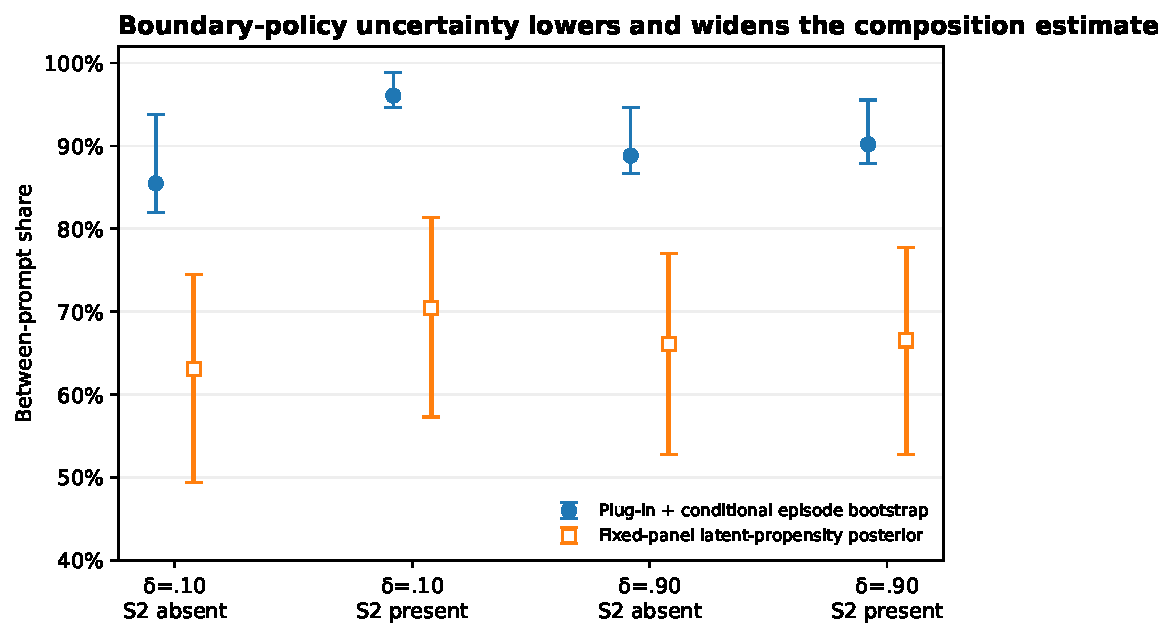
\includegraphics[width=.95\linewidth]{figures/between-prompt-share.pdf}}

\emph{Figure S1. Between-prompt share of episode-level variation. The
Jeffreys fixed-panel posterior propagates uncertainty in six-episode
prompt cells; plug-in/conditional-bootstrap estimates describe the
archived concentration more literally. A symmetric-prior sweep reported
in text shows that the stronger ``share above one-half'' interpretation
is prior-dependent.}

Across the represented continuation-probability treatment, the observed
fixed-panel point differences are +0.083 for S2-absent wording and
+0.078 for S2-present wording. Conservative exact simultaneous 95\%
intervals are {[}−0.171, +0.330{]} and {[}−0.181, +0.330{]}. Their
breadth jointly reflects the registered six-episode-per-cell design and
an exact projection that retains non-zero uncertainty at empirical
corners. The treatment changes both the continuation process and the
text used to communicate it; round-one actions identify response under a
specified representation, not a semantically neutral economic parameter.
The point estimates are small on the unit scale, but the data do not
establish equivalence, a zero response, or a narrow upper bound.

The empirical point is not that six repeated episodes should have
produced high precision. It is that the registered marginal criteria did
not require the treatment-response object to be estimated precisely, yet
their passage could be read as validation; the intervals quantify what
that validation design left unidentified. For the finite archived panel,
+0.083 and +0.078 are exact descriptive arithmetic. A design-effect
heuristic using six episodes per prompt and the plug-in between-share
range 0.855--0.961 gives roughly 16.5--18.2 episode equivalents per
condition, close to the sixteen prompt units. This is not the degrees of
freedom of the exact procedure, but it identifies prompt-family size as
the operative precision constraint. Figures 2--3 show the prompt-indexed
contrasts and fixed-panel condition means.

\pandocbounded{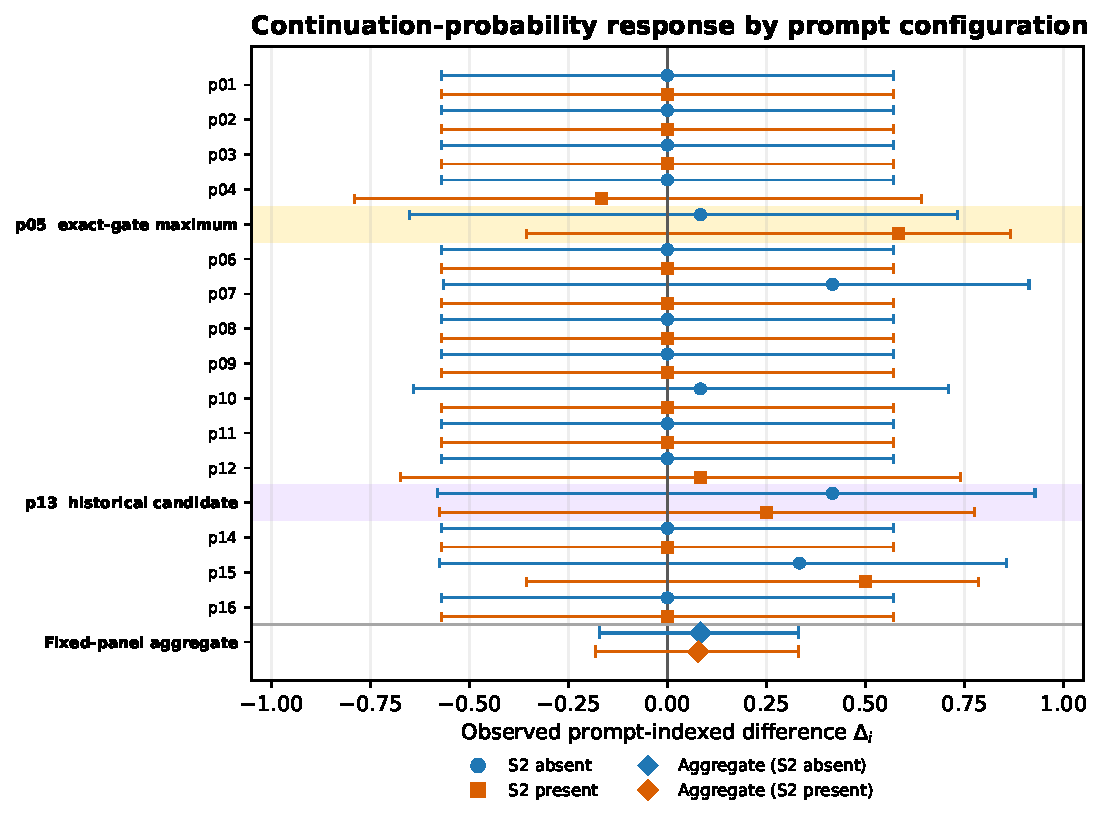
\includegraphics[width=.95\linewidth]{figures/prompt-indexed-delta.pdf}}

\emph{Figure S2. Prompt-indexed differences in round-one cooperation,
\(\Delta_i=\hat p_i(\delta=.90)-\hat p_i(\delta=.10)\), for both wording
families. Bars are conservative exact simultaneous 95\% intervals with
complete episodes as the unit; observed corners retain non-zero
uncertainty. The p05 row is flagged as the largest candidate eligible
under the conservative exact family gate, and p13 as the historical
candidate selected by the original rule.}

\pandocbounded{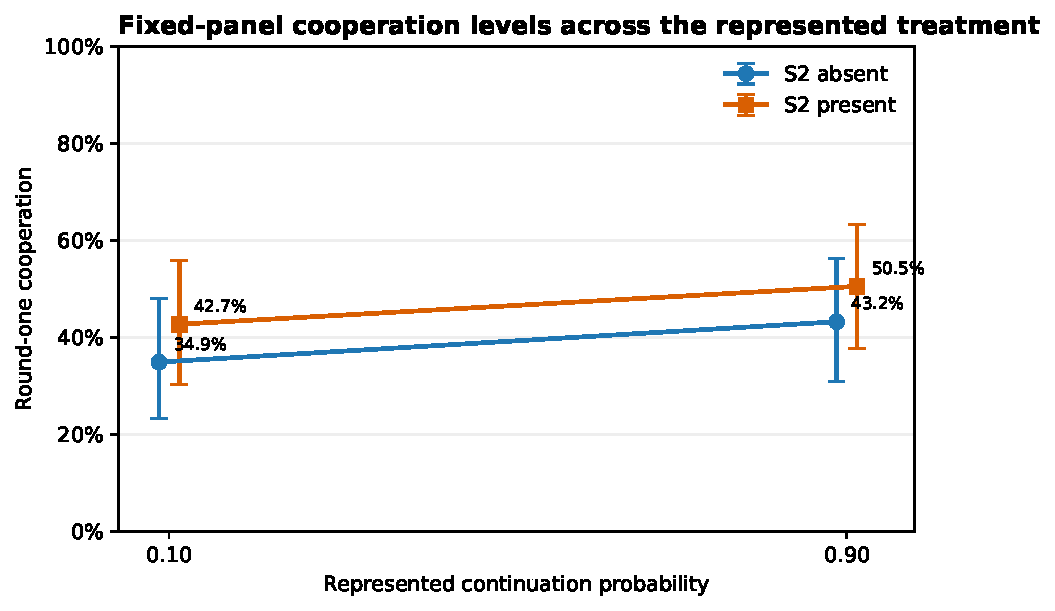
\includegraphics[width=.95\linewidth]{figures/condition-means.pdf}}

\emph{Figure S3. Fixed-panel cooperation by represented
continuation-probability condition. Error bars are conservative exact
condition intervals; lines connect conditions for orientation only.}

The broad-reference cooperation band was {[}0.36, 0.63{]}. Repeated-game
pool means were 0.349, 0.427, 0.432, and 0.505; only the S2-absent
\(\delta=.10\) cell fell outside, by 0.011 below the lower boundary. The
preregistered leaning rule divides the panel into eight
cooperative-leaning and eight defect-leaning complete prompts.
Descriptive gaps range from 0.510 to 0.719 across the repeated-game
conditions and are fixed-panel prompt-bundle contrasts, not causal trait
effects:

\textbf{condition:} \texttt{rep-d10-s2a}; \textbf{cooperative-leaning
mean:} 0.615; \textbf{defect-leaning mean:} 0.083; \textbf{difference:}
+0.531; \textbf{prompts per stratum:} 8

\textbf{condition:} \texttt{rep-d10-s2p}; \textbf{cooperative-leaning
mean:} 0.760; \textbf{defect-leaning mean:} 0.094; \textbf{difference:}
+0.667; \textbf{prompts per stratum:} 8

\textbf{condition:} \texttt{rep-d90-s2a}; \textbf{cooperative-leaning
mean:} 0.688; \textbf{defect-leaning mean:} 0.177; \textbf{difference:}
+0.510; \textbf{prompts per stratum:} 8

\textbf{condition:} \texttt{rep-d90-s2p}; \textbf{cooperative-leaning
mean:} 0.865; \textbf{defect-leaning mean:} 0.146; \textbf{difference:}
+0.719; \textbf{prompts per stratum:} 8

\textbf{condition:} \texttt{os-community}; \textbf{cooperative-leaning
mean:} 0.688; \textbf{defect-leaning mean:} 0.019; \textbf{difference:}
+0.669; \textbf{prompts per stratum:} 8

P5-1b used protocol-nonmatched human SD references mechanically implied
from Dal Bó and Fréchette's (2011) R=40 strategy-frequency estimates:
0.4122 for their \(\delta=.50\) panel and 0.3116 for \(\delta=.75\). The
frozen ratio \(\rho=.75\) gave thresholds 0.3092 and 0.2337. It was a
preregistered heuristic tolerance, not an equivalence margin.
Finite-opportunity-corrected plug-in SDs were 0.4182, 0.4784, 0.4408,
and 0.4323. A conditional episode bootstrap produced corrected-SD
intervals {[}0.4122, 0.4391{]}, {[}0.4696, 0.4916{]}, {[}0.4279,
0.4654{]}, and {[}0.4269, 0.4496{]}, but unanimous cells remain point
masses in that bootstrap. The first lower bound was independently
reproduced at full precision; its displayed equality to the 0.4122 human
reference is a rounding coincidence. A two-stage prompt+episode
bootstrap changes the estimand toward a hypothetical persona generator
and yields wider SD intervals {[}0.2724, 0.4879{]}, {[}0.3696,
0.5123{]}, {[}0.3457, 0.4890{]}, and {[}0.3345, 0.4847{]}. P5-1b is
therefore retained as a permissive historical checkpoint, not evidence
of human-variance equivalence.

Across all six Phase 5 conditions, the historical seat-level rule
classifies 14/96 persona-condition cells interior, the exact episode
projection 11/96, and the Jeffreys sensitivity 19/96. In the registered
32-unit set, the counts are 3/32, 2/32, and 5/32. At \(n=6\) with a
three-valued outcome, modest differences in interval width move cells
across the threshold; continuous uncertainty and variance components are
more informative than the binary census.

Descriptively, the composition pattern did not transfer to the
endpoint-nonstationary Gemini tier: 9/24 Gemini cells met the historical
interiority rule versus 14/96 in the primary panel, and several
representation effects reversed direction. This is consistent with
deployment-specific composition; the tier is not a formal replication.
Human references remain protocol-nonmatched because continuation
probabilities, payoffs, incentives, assignment, and experience differ
from the present design; no matched magnitude or human-equivalence claim
is made.

\subsubsection{S3.2 Representation interventions expose prompt-surface
control}\label{s3.2-representation-interventions-expose-prompt-surface-control}

For the bare configuration, round-one cooperation was 0.000 at every
registered continuation probability. X2 decomposed the v1 and v2a prompt
bundles into six sentence/block spans and constructed forward and
reverse ladders by replacing one complete span at a time. The selected
S2 operation replaced and repositioned ``After every round there is a
\{deltaPct\}\% chance the session continues with another round'' with
``At the end of each round there is a \{deltaPct\}\% chance that the
session goes on for one more round.'' Screening used ten episodes per
rung; the selected minimal pair was confirmed at temperature 0.7 on 20
fresh episodes per side (seeds 2953--2972), moving cooperation from 0/40
to 37/40. Because wording and position were one atomic operation, the
design does not separate them.

The effect was specific to the representation of repeated interaction,
not a generic main effect of wording. In the 640-episode one-shot D1
battery, GPT-4.1's registered wording main effect was +0.0063 (SE
0.0210; Holm-adjusted \(p=1.00\)), and none of the registered wording
interactions was supported. Conversely, the D1 presentation selected for
the repeated assay had a one-shot mean of 0.100; when embedded in the
repeated-game protocol, round-one cooperation rose to 0.750 at
\(\delta=.10\) and 1.000 at \(\delta=.90\). The Community wrapper
produced 1.000 in both conditions. These repeated cells were correctly
classified as ceiling-confounded, so they do not identify a
continuation-probability slope. They do show that announcing and
implementing repeated interaction can be a much larger treatment than
ordinary one-shot wording variation.

In the label-swap cell, canonical payoffs were held fixed while
``Cooperate'' and ``Defect'' were attached to opposite strategic roles.
The bare configuration chose the cooperation-worded option 0/40 times
and instead took the payoff-dominated role whenever it carried the word
``Defect.'' This shows that the displayed label or a label-linked
learned prior can override payoff dominance in this registered cell. It
does not identify intrinsic lexical valence: a learned game-theoretic
association such as ``Defect = equilibrium/dominant action in Prisoner's
Dilemma'' is an equally plausible mechanism. A structurally equivalent
non-PD control retaining the same labels was not run.

Persona conditioning produces two observed contrasts, but they are not
factorially separable. Differences among complete persona prompts
generate the leaning gaps reported in S3.1. Adding any tested persona
string reverses the bare swap-cell choice, yet no non-semantic prefix
matched for length, punctuation, and position was run; semantic persona
content cannot be isolated from generic sequence-format disruption. In
the swap cell, label and payoff also point to the same option for
persona-conditioned configurations, leaving the reversal mechanism
ambiguous.

P5-3(b)'s 24 evaluable lanes comprise sixteen personas at T=0.7 plus
p02, p06, p11, and p15 at each of T=1.0 and T=1.3. Every lane retains a
simultaneous episode-exact lower bound above the frozen 0.20 threshold;
the minimum is 0.462. The pooled P5-2 task-consistent share is 90/704
seat decisions across 352 episodes, equivalently 45/352=0.128 on episode
means. The frozen historical adjudication used the seat-level rule. An
episode-iid Clopper--Pearson projection gives {[}0.092, 0.172{]}, but
that interval does not propagate the prompt clustering visible elsewhere
in the study. A post-adjudication stratified prompt-cluster bootstrap
over the forty registered persona × conflict-cell clusters preserves the
empirical point estimate and gives 95\% interval {[}0.071, 0.189{]}.

Independent fixed-panel Dirichlet aggregation is materially
prior-sensitive because every sparse cluster receives its own symmetric
prior. Under the Jeffreys specification, each cluster receives total
prior concentration 1.5, or 60 category-count units across forty
clusters; this is not literally equivalent to sixty pooled episodes
because the clusters have unequal sizes, but it is non-negligible
relative to 352 observations and pulls the aggregate toward 0.5. A
zero-call sensitivity sweep gives:

\textbf{symmetric \(\alpha\):} 0.10; \textbf{posterior median:} 0.138;
\textbf{95\% interval:} {[}0.124, 0.153{]};
\textbf{\(P(\theta\le .20)\):} 1.000

\textbf{symmetric \(\alpha\):} 0.25; \textbf{posterior median:} 0.152;
\textbf{95\% interval:} {[}0.135, 0.171{]};
\textbf{\(P(\theta\le .20)\):} \textgreater0.999

\textbf{symmetric \(\alpha\):} 0.50; \textbf{posterior median:} 0.172;
\textbf{95\% interval:} {[}0.152, 0.195{]};
\textbf{\(P(\theta\le .20)\):} 0.991

\textbf{symmetric \(\alpha\):} 1.00; \textbf{posterior median:} 0.205;
\textbf{95\% interval:} {[}0.182, 0.231{]};
\textbf{\(P(\theta\le .20)\):} 0.329

The Jeffreys posterior's proximity to the registered 0.20 boundary is
therefore prior-dependent rather than an independent signal from the
data; the \(\alpha=1\) posterior crosses the boundary. The
prompt-cluster bootstrap is the principal dependence-aware sensitivity.
Every repeated conflict subcell is mixed; only the swap cell is
individually persona-dominant. The historical pooled classification is
therefore mechanism-confounded and carried by the swap cell, not
evidence of a general persona-dominance mechanism. Figure S4 summarizes
the two bare-configuration representation interventions.

\pandocbounded{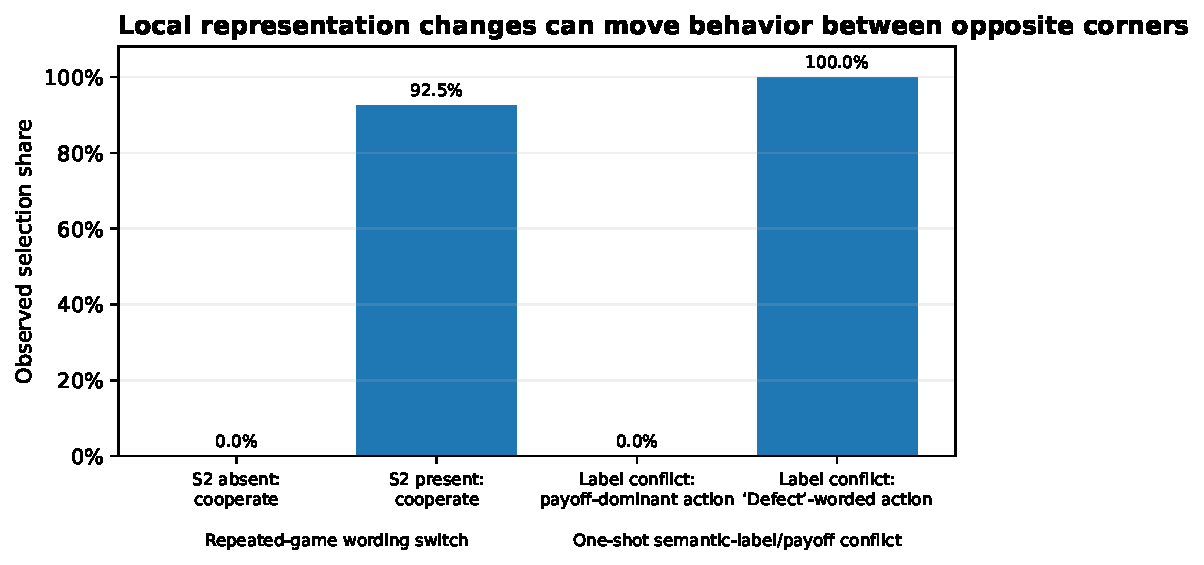
\includegraphics[width=.95\linewidth]{figures/representation-effects.pdf}}

\emph{Figure S4. Two representation interventions in the bare
configuration. The S2 wording-and-position operation moved cooperation
from 0/40 to 37/40. In the one-shot label conflict, the payoff-dominant
action was never chosen when the dominated role carried ``Defect.''
These bars report selection shares, not a common or uniquely identified
causal mechanism.}

\subsubsection{S3.3 What the marginal checks cannot
identify}\label{s3.3-what-the-marginal-checks-cannot-identify}

Let \(p_i(d)=E[Y\mid i,d]\), where \(i\) indexes the complete explicit
persona prompt and \(d\) the experimental condition.

\textbf{Proposition A: broad bands only partially identify the aggregate
contrast.} If a synthetic condition mean is accepted within tolerance
\(\epsilon_d\) of a reference mean in each condition, then

\[|\Delta^S-\Delta^H|\le \epsilon_0+\epsilon_1.\]

Equivalently, accepted bands \([\ell_0,u_0]\) and \([\ell_1,u_1]\) imply
only

\[\Delta^S\in[\ell_1-u_0,u_1-\ell_0].\]

Exact condition-specific mean matching would force the aggregate effect
by the identity \(\Delta=\mu_1-\mu_0\); the empirical failure lives in
the slack of coarse criteria.

\textbf{Proposition B: aggregate moments do not identify microstructure
or response coupling.} This is an application of the law of total
variance and classical Fréchet--Hoeffding/Sklar coupling results
(Hoeffding 1940; Sklar 1959) to synthetic-participant validation, not a
new probability theorem. Mean and total variance do not identify how
variation is divided between prompt configurations and repeated draws,
nor do they identify distributional shape or boundary concentration.
Even exact condition-specific distributions do not identify the
cross-condition coupling and therefore do not identify the distribution
of prompt-indexed responses \(\Delta_i=p_i(1)-p_i(0)\). Reusing an
explicit persona string supplies one prompt-indexed coupling, but
interpreting it as a stable synthetic individual's potential-outcome
contrast requires latent-person invariance, which this study does not
test.

The study therefore identifies a composition pattern in one fixed prompt
panel. It does not establish that humans have a different
microstructure, that RLHF caused the pattern, that latent-user drift is
absent, or that the same pattern occurs across persona generators.

\subsubsection{S3.4 The favored persona-level result is not
prospectively confirmed; the archived family is
underpowered}\label{s3.4-the-favored-persona-level-result-is-not-prospectively-confirmed-the-archived-family-is-underpowered}

Under the historical seat-level rule, persona p13 moved from 0.333
cooperation at δ=.10 to 0.750 at δ=.90 and passed a per-candidate
lower-bound test. The rule searched multiple persona × wording
candidates and fired on any pass without declared family-level error
control. External review identified that defect.

Three 200,000-permutation gate constructions are now reported; all
permutation p-values use the add-one convention,
\(\widehat p=(r+1)/(B+1)\), with exact Monte Carlo intervals. Under the
historical seat-level gate, p13 remains the maximum at +0.4167, with
familywise \(p=0.059230\), Monte Carlo 95\% interval {[}0.058194,
0.060268{]}. Under the percentile episode-cluster-bootstrap sensitivity,
p13 also remains the maximum and \(p=0.043455\), interval {[}0.042561,
0.044353{]}. The exact projection is the conservative reference because
it has finite-sample coverage for the discrete episode mean; the
percentile bootstrap is retained symmetrically but has no comparable
small-sample coverage guarantee. Under the conservative exact-episode
gate, p13 is ineligible: its low-δ lower bound falls below 0.05 and its
high-δ upper bound exceeds 0.95. Only p04/s2p and p05/s2a pass both
gates; the largest eligible slope belongs to p05/s2a (+0.0833), with
familywise \(p=0.773206\), interval {[}0.771363, 0.775039{]}.

For p13/s2a, the percentile bootstrap admitted both conditions as
interior---δ=.10: {[}0.083, 0.667{]}; δ=.90: {[}0.583,
0.917{]}---whereas the conservative exact projection rejected
both---{[}0.047, 0.800{]} and {[}0.287, 0.954{]}, respectively. Neither
recorded cell was at an exact corner. The eligibility difference
therefore arises from small-sample interval width and coverage behavior,
not from a corner interval falsely passing the gate.

The complete data-dependent gate is dynamically reapplied within every
permutation, not frozen from the observed-data mask. The implementation
precomputes 56 possible-composition gate values and performs 25,600,000
condition-gate lookup applications at B=200,000. In a deliberately
incorrect comparison that froze the observed-data mask, the maximum
statistic differed from the dynamic procedure in 718 of 5,000 null draws
(14.4\%), showing that reapplication materially changes the reference
distribution. Lookup/direct parity and the frozen-mask regression are
included in the public audit record (S4).

An exhaustive attainability audit shows that, with six episodes per
condition, 12 of the 28 possible episode-value compositions pass the
exact gate. Their sample means range from 0.333 to 0.667, but
eligibility depends on the full \({0,0.5,1}\) composition rather than on
the mean alone. Two eligible cells can therefore differ by at most
0.333. Under the archived 32-candidate null structure, the add-one
familywise tail probability at that maximum attainable slope is
0.075040, with Monte Carlo 95\% interval {[}0.073884, 0.076198{]}; no
exact-gate result in this archived family can reach 0.05. The exact
analysis is therefore a valid dependence-aware sensitivity but not a
powered disconfirmation of a p13-sized capability claim. The record
neither prospectively confirms nor decisively disconfirms p13; it
identifies a replication target whose next test must be sized
prospectively (S5.3). A separately authorized prospective test could
preregister the candidate family, episode-level dependence unit,
interiority gate, maximum statistic, familywise decision rule, and
sample size before any data are collected.

These variants were specified and executed together only after external
review exposed the original defects. No familywise gate was registered
at the original freeze, and the repository contains no
seal-before-compute record for these sensitivities. The analyses ran in
GitHub Actions against archived databases with fixed seeds, and their
outputs were committed regardless of direction. Accordingly, the
favorable \(p=0.043455\) variant cannot create prospective confirmation,
just as the other variants cannot retroactively strengthen the frozen
claim. The historical mechanical P5-3 verdict remains visible because
clause (b) fired strongly and p13 passed the rule as frozen. Clause (a)
did not prospectively establish the capability claim because the frozen
search lacked family control; the conservative post-adjudication
procedure is too underpowered at n=6 to provide decisive evidence
against it. Figure S5 compares the three post-adjudication familywise
constructions and their different eligibility rules.

\pandocbounded{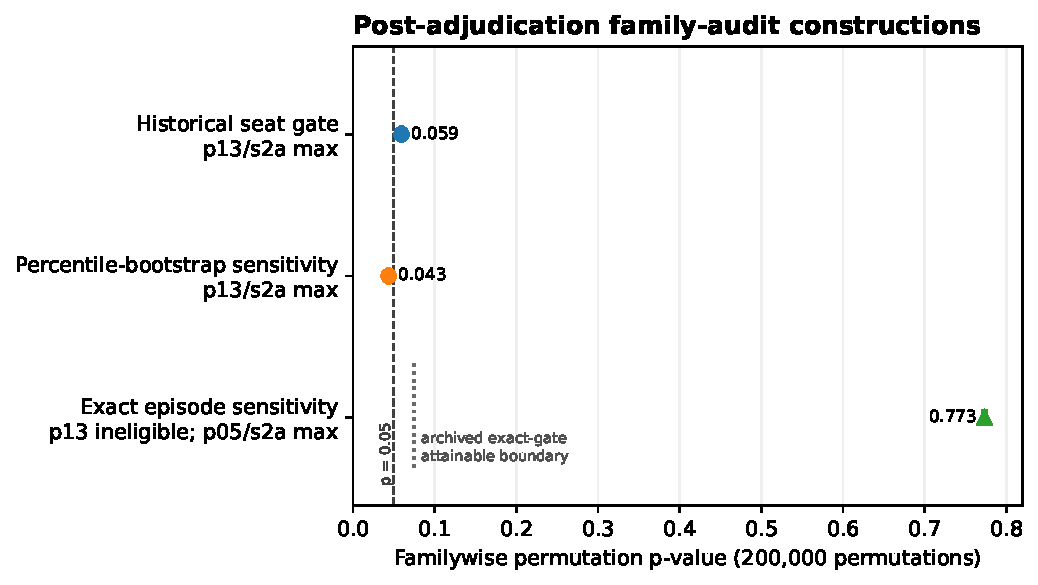
\includegraphics[width=.95\linewidth]{figures/p13-audit.pdf}}

\emph{Figure S5. Post-adjudication familywise constructions. The first
two points are p13/s2a under the historical and percentile-bootstrap
gates. Under the conservative exact-episode gate, p13 is ineligible; the
third point is the familywise result for the largest eligible candidate,
p05/s2a. The dotted line at \(p=0.075040\) marks the estimated minimum
attainable familywise p-value for the archived \(n=6\), 32-candidate
exact-gate design and applies only to that construction. None of the
procedures was registered at the original freeze; see S3.4 for the
bounded scientific status.}

\subsubsection{S3.5 Auditability}\label{s3.5-auditability}

Twelve registered author predictions were refuted by data and published.
Four underspecified analysis choices were resolved outcome-blind. A
two-sided gate blocked a false ceiling conclusion. Sentinels detected a
time-indexed behavioral discontinuity in an unversioned endpoint and
exposed a monitoring gap that was repaired with an attestation gate. The
public capsule now verifies all 4,916 confirmatory Phase 3--5 runs with
zero live model calls: 4,896 LLM runs replay byte-exact and 20
deterministic baselines are independently recomputed. External review
then found the family-error and dependence defects discussed above; the
archived record made both diagnosable and correctable.

The claim is bounded: the machinery is procedurally exact and
extensively auditable. Its strongest achievement is not self-validation
but preservation of enough provenance for outsiders to identify where
procedural correctness stopped short of statistical validity.

\subsection{S4. Data availability and replay
limits}\label{s4.-data-availability-and-replay-limits}

The public repository contains the event stores, prompt registries,
sealed registrations, adjudication records, timestamp proofs,
post-adjudication analyses, figures, manuscript history, and review
record. The one-command capsule verifies all 4,916 confirmatory Phase
3--5 runs with zero credentials and zero live model calls. The audit
covers 320 registered Phase 3/X1 LLM runs, 20 deterministic Phase 3
baselines, 2,864 Phase 4 runs, and 1,712 Phase 5 runs; three additional
completed legacy entry/diagnostic runs are also replayed but are not
counted as confirmatory. Phase 3 replay re-renders every prompt,
requires recorded-cache hash hits, reparses raw completions, recomputes
actions, payoffs, and RNG draw counts, and checks recorded call parity.
The deterministic P3-C3 baseline is independently recomputed from
archived seeds and game objects.

Phase 3 used a legacy provider path without Phase 4--5 response IDs or
deterministic request-body SHA capture. Phase 4--5 contain 30,421 normal
request events and 30,397 response events; the 24-event difference is
the disclosed provider-failure partial set. Each partial belongs to a
failed run, was excluded from completed-run analyses and the 4,916-run
replay denominator, and was never decoded as an action. Request attempts
remain represented in request and budget accounting rather than being
silently discarded; only completed replacement runs, where present under
the registered replacement procedure, enter analysis. Those response
records contain rendered prompts, bundle and request-body hashes, engine
commit and provider route, raw text, and provider response IDs.
Individual completion payloads were not provider-attested or separately
hash-chained at receipt. Capsule checksum manifests and external
timestamps make the released database snapshot tamper-evident relative
to publication; replay cannot prove that no alteration occurred before
snapshot sealing.

Reproduce the confirmatory record with:

\begin{verbatim}
git clone https://github.com/yoheinakajima/synthetic-players
cd synthetic-players/capsule
bash verify.sh
\end{verbatim}

All post-adjudication analyses are zero-call scripts over the archived
databases and are labeled separately from prospectively registered
results. The principal machine-readable surfaces are the Submission
Analyses directory (count reconciliation, dependence sensitivities,
family audits, and the final prior sweep), the Persona Table, the
Literature Map and Novelty Relationships documents, and the Review
Archive. Stable links to each are provided from the repository's review
entry point, keeping the empirical argument readable without embedding
long filesystem paths in the paper.

Journal preparation used the native replay audit functions in process,
avoiding the historical HTTP transport. The original 190-file capsule
manifest passed before and after. The receipt and reports are supplied
under \texttt{evidence/}; this was an offline recheck, not a new model
run. Python 3.11.15 differs from the historical environment note
3.11.14. Both identities remain documented. The README line that ends at
4,916 omits three legacy diagnostics; the verifier covers 4,919 (4,899
LLM plus twenty baselines), including 4,916 confirmatory. Earlier
4,576-run hierarchy/review descriptions refer to an earlier boundary.

\subsection{S5. Retained secondary results and optional future
work}\label{s5.-retained-secondary-results-and-optional-future-work}

\subsubsection{S5.1 Temperature
secondary}\label{s5.1-temperature-secondary}

Choice entropy is defined as base-2 Shannon entropy,
\(H=-\sum_a p(a)\log_2p(a)\), over round-one payoff-role choices. The
historical registered secondary pooled all valid choices at each
temperature, but the T=0.7 and higher-temperature samples had different
composition. The matched-sweep reanalysis uses only persona-cell lanes
observed at all three temperatures:

\textbf{temperature:} 0.7; \textbf{matched units:} 13; \textbf{seats:}
544; \textbf{pooled Shannon entropy (bits):} 0.8310; \textbf{mean
within-unit entropy (bits):} 0.4484

\textbf{temperature:} 1.0; \textbf{matched units:} 13; \textbf{seats:}
284; \textbf{pooled Shannon entropy (bits):} 0.7822; \textbf{mean
within-unit entropy (bits):} 0.2566

\textbf{temperature:} 1.3; \textbf{matched units:} 13; \textbf{seats:}
284; \textbf{pooled Shannon entropy (bits):} 0.7698; \textbf{mean
within-unit entropy (bits):} 0.2877

The registered pooled decline is partly composition-confounded but
survives on the identical sweep lattice. Mean within-unit entropy is
reported separately because pooled entropy can remain high when
different prompt-cell units occupy opposite boundaries. Neither
statistic identifies a temperature mechanism. The plug-in Shannon
estimates use unequal seat counts (544 versus 284 and 284), so their
small finite-sample biases are not identical; no bias-corrected entropy
claim is made.

\subsubsection{S5.2 Other supplementary
findings}\label{s5.2-other-supplementary-findings}

The following registered or explicitly descriptive results are outside
the paper's main composition--response arc but are retained here so that
the completed experimental record is citable.

\textbf{Opponent-contingent adversarial play.} In the 50-round RPS
adversary suite, a second-order n-gram opponent earned +0.215 payoff
units per round against GPT-4.1 and survived Holm correction. A
first-order tracker instead earned -0.118, meaning the subject beat it.
The WSLS-targeter, designed around the earlier near-deterministic
lose-shift signature, earned only +0.008 with a lower confidence bound
below zero, although it outperformed the first-order tracker by +0.126.
The shuffled-history control was not worse than the ordered tracker.
Thus a behavioral signature measured against one opponent did not
transport as a simple profitable rule against another; exploitable
structure was opponent-contingent rather than captured by a single
global label. The GPT-4.1 opponent tests were registered; the six
secondary arm tests were Holm-controlled, while the cross-opponent
transport interpretation here is descriptive.

\textbf{Role-attached asymmetry in a symmetric game.} After RPS moves
were renamed with neutral symbols and display order was exactly
counterbalanced, the registered GPT-4.1 first-minus-rock contrast was
-0.181: the preregistered positive-direction hypothesis was not
supported, and the observed direction was reversed. A support-only
Dirichlet analysis assigned probability 0.0001 to first-only selection
exceeding rock-only selection. The cross-vendor mirror had the opposite
sign, +0.243, with a one-sided lower bound of +0.139. The GPT-4.1
contrast was registered; the Gemini mirror is reported descriptively
under the paper's cross-vendor tier. The pattern is descriptive evidence
of vendor-specific, role-attached asymmetry in a formally symmetric
game, not a universal ``rock bias.''

\textbf{Cross-vendor label--payoff dissociation.} In the canonical
label-swap cell, GPT-4.1 chose the cooperation role 1.000 of the time
while choosing the displayed word COOPERATE 0.000, thereby following the
displayed token DEFECT even when it named the payoff-dominated role.
Gemini chose the cooperation role 0.213 and the word COOPERATE 0.788,
mostly following the payoff-dominant role instead. When counterfactual
payoffs made the cooperation role strictly dominant and displayed it as
DEFECT, the two models' cooperation-role shares were 1.000 and 0.975.
For GPT-4.1, word and payoff dominance were congruent in this cell, so
it does not separate the two channels. For Gemini, the cell is
informative because the model moved to the payoff-dominant cooperation
role despite that role carrying DEFECT. The GPT-4.1 cells were
registered; the Gemini figures are descriptive under the paper's
cross-vendor tier. The vendors differed in when a familiar action word
overrode the supplied payoff structure; the data do not identify one
universal lexical mechanism.

\textbf{Endpoint drift and subject eligibility.} The Gemini sentinel
fingerprint changed from 10/10 baseline matches to a sequence reaching
6/10 and 7/10 on the unversioned endpoint, triggering freezes,
disclosure, re-baselining, and a later attestation gate. GPT-4.1's
sentinel cells remained 10/10. Separately, Claude Haiku failed the
registered behavioral entry gate and was replaced through a sealed
amendment. This is a procedural record, not a behavioral-effect
estimate. Together the cases show that model identity and endpoint
availability do not by themselves establish a stable, usable behavioral
subject.

\subsubsection{S5.3 Prospective
replication}\label{s5.3-prospective-replication}

A separately authorized prospective replication could preselect one
target or a small candidate family and preregister the complete
familywise procedure: candidate set, episode-level unit, interiority
gate, maximum statistic, decision threshold, and sample size. For the
composition estimand, it will either widen the preregistered prompt
family or prospectively sample from a declared persona generator rather
than reuse the fixed sixteen prompts as if they represented a
population. For the response estimand, the episode allocation will be
chosen by simulating the exact registered gate and candidate family
until the minimum attainable familywise p-value is below the declared
threshold and power meets a prespecified target under the declared
alternative. The design should also include a format-matched neutral
prefix, a continuation-probability × wording factorial, and a
structurally equivalent non-PD label-conflict control.

\subsubsection{S5.4 Research record}\label{s5.4-research-record}

The complete correction ledger, sealed discussion text, dead-predictions
ledger, reviewer-role disclosures, and mechanical disposition matrices
are maintained in the public Review Archive and Submission Analyses
directories. Persona provenance is documented in the Persona Table;
scholarly positioning is documented in the Literature Map and Novelty
Relationships documents. Historical artifacts are never silently
rewritten; current interpretations are linked to the versions they
amend.

\subsection{S6. Sealed discussion in
full}\label{s6.-sealed-discussion-in-full}

The following historical text is reproduced for provenance. It is
superseded where the main article and S3 withdraw its capability
interpretation. Its header and prediction errors are part of the sealed
record.

\section{Paper one --- pre-committed discussion branches (Phase
5)}\label{paper-one-pre-committed-discussion-branches-phase-5}

\begin{quote}
\textbf{STATUS: PROPOSED --- UNSEALED.} This file seals (hash-anchored
with registry v4) BEFORE any Phase 5 dispatch. After seal it is
immutable: the published paper's discussion section must be
byte-diffable against the branch the registered verdicts select. The
author does not get a vote after data exists. The completeness linter
(check C5) treats a registered verdict combination without a written
branch as a seal failure.
\end{quote}

\subsection{Verdict axes and branch-selection rule
(registered)}\label{verdict-axes-and-branch-selection-rule-registered}

Three registered verdict axes select the branch:

\begin{itemize}
\tightlist
\item
  \textbf{A} --- P5-1 corner mixture: \texttt{supported} /
  \texttt{not-supported}
\item
  \textbf{B} --- P5-3 interior persona existence: \texttt{zero} /
  \texttt{at-least-one}
\item
  \textbf{C} --- P5-4 temperature refutation (interior fraction rises
  with T, or a payoff-graded response appears at high T): \texttt{no} /
  \texttt{yes}
\end{itemize}

Selection rule, applied in this order: if \textbf{B = at-least-one} →
Branch 2. Else if \textbf{C = yes} → Branch 3. Else if \textbf{A =
supported} → Branch 1. Else → Branch 4.

P5-2 (surface-cue dominance hierarchy) does not select the branch; every
branch contains both pre-written P5-2 variant paragraphs (task-dominant
/ not task-dominant) and the published text keeps exactly the variant
the P5-2 verdict selects.

\subsubsection{Combination table (exhaustive;
linter-checked)}\label{combination-table-exhaustive-linter-checked}

\textbf{A (P5-1):} supported; \textbf{B (P5-3):} zero; \textbf{C
(P5-4):} no; \textbf{Branch:} Branch 1 --- corners everywhere

\textbf{A (P5-1):} supported; \textbf{B (P5-3):} zero; \textbf{C
(P5-4):} yes; \textbf{Branch:} Branch 3 --- temperature-graded

\textbf{A (P5-1):} supported; \textbf{B (P5-3):} at-least-one; \textbf{C
(P5-4):} no; \textbf{Branch:} Branch 2 --- an interior persona exists

\textbf{A (P5-1):} supported; \textbf{B (P5-3):} at-least-one; \textbf{C
(P5-4):} yes; \textbf{Branch:} Branch 2 --- an interior persona exists

\textbf{A (P5-1):} not-supported; \textbf{B (P5-3):} zero; \textbf{C
(P5-4):} no; \textbf{Branch:} Branch 4 --- mixed

\textbf{A (P5-1):} not-supported; \textbf{B (P5-3):} zero; \textbf{C
(P5-4):} yes; \textbf{Branch:} Branch 3 --- temperature-graded

\textbf{A (P5-1):} not-supported; \textbf{B (P5-3):} at-least-one;
\textbf{C (P5-4):} no; \textbf{Branch:} Branch 2 --- an interior persona
exists

\textbf{A (P5-1):} not-supported; \textbf{B (P5-3):} at-least-one;
\textbf{C (P5-4):} yes; \textbf{Branch:} Branch 2 --- an interior
persona exists

\begin{center}\rule{0.5\linewidth}{0.5pt}\end{center}

\subsection{Branch 1 --- corners
everywhere}\label{branch-1-corners-everywhere}

The question Phase 5 asked was whether any conditioning of the subject
--- content-side, through persona system prompts, or decoding-side,
through temperature --- could produce a human-like interior behavioral
population. The answer is no. Sixteen personas generated by a seeded
procedure from crossed trait factors, evaluated across the program's
main instruments at three temperatures, produced pools that are mixtures
of the same corners the bare subject occupies: the fraction of
persona-cells with interior episode-level cooperation stayed below the
registered threshold, and between-persona variance fell short of the
published human within-condition panels cited in the sealed predicates.
Personas relocate the corners and decorate them with demographic
texture; they do not populate the interior between them.

This completes the program's central claim in its strongest available
form. Phases 3 and 4 established that the bare subject's behavior is
driven by local semantic-textual content rather than payoffs or display
mechanics. Phase 5 shows the result is not an artifact of the bare
subject's blankness: no member of a registered persona population passed
the two-sided assay gate with a positive discount-factor slope, and none
refused the dominated mislabeled option at the registered rate.
Incentive sensitivity --- the signature of economic agency that every
human panel in the cited literature exhibits at the individual level ---
did not appear anywhere in the conditioned population, at any
temperature.

\emph{P5-2 variant (task-dominant):} The dominance hierarchy sharpens
the mechanism. Where a persona's registered leaning conflicted with the
known task-text switches, the task text won at the registered margin:
local semantic content beats global framing one layer up, exactly as the
Phase 4 thesis predicted. The system prompt is weaker than the words in
front of the model.

\emph{P5-2 variant (not task-dominant):} The dominance hierarchy did not
resolve at the registered margin: in conflict cells, persona leaning and
task-text switches produced mixed control of choice. This bounds the
Phase 4 thesis --- local semantic content dominates the bare subject,
but a global persona frame can contest it --- without disturbing the
corner-mixture result, which held regardless of which cue won.

Temperature behaved as registered: raised T manufactured variance ---
symmetric flip-noise around the corners and elevated invalid rates ---
without manufacturing behavior. The interior fraction did not increase,
and no payoff-graded response appeared at any temperature. For
simulation practice the implication is direct and negative:
persona-conditioning and decoding heat, the two levers practitioners
actually pull to make synthetic subjects ``diverse,'' produce
populations that are diverse in costume and uniform in mechanism.
Synthetic-player pools built this way cannot substitute for human panels
in any design where interior heterogeneity or incentive sensitivity
carries the identification.

\subsection{Branch 2 --- an interior persona
exists}\label{branch-2-an-interior-persona-exists}

The headline of Phase 5 is an existence result the program registered
against itself: at least one persona in the sealed sixteen passed the
two-sided assay gate and showed the registered signature of incentive
sensitivity. The author's registered prediction --- that none would ---
is refuted, and the refutation is the finding. Human-likeness, absent in
the bare subject throughout Phases 3 and 4, can be relocated into the
conditioning layer: some region of persona space induces interior
behavior with a positive discount-factor slope (or registered-rate
refusal of the dominated mislabeled option), where the bare subject
shows corners and surface-cue tracking.

Which persona(s) passed, and their registered trait factors, are
reported in the results section exactly as adjudicated; nothing in this
pre-committed text depends on which cell cleared the gate. What the
existence result changes is the interpretation of the program's earlier
phases: the corner behavior of Phases 3--4 characterizes the bare
subject, not the model's capability envelope. The capability was
recoverable by content-side conditioning that contains no game-relevant
instruction --- trait words only, under the sealed banned-content guard.

\emph{P5-2 variant (task-dominant):} Even so, the dominance hierarchy
held where tested: in registered conflict cells, task-text switches beat
persona leaning at the registered margin. Interior behavior and
surface-cue dominance coexist --- conditioning moved the operating point
without transferring control from local semantic content to the global
frame.

\emph{P5-2 variant (not task-dominant):} Consistent with the existence
result, the dominance hierarchy did not resolve for the task side:
persona framing contested or beat the task-text switches in registered
conflict cells. The two results together indicate that the system-prompt
layer is not inert decoration but a genuine second channel of behavioral
control.

The scope of the claim is deliberately narrow. One (or few) passing
persona(s) out of sixteen is not a human-like population; the population
predicates (P5-1) are reported alongside, and the between-persona
variance comparison against the cited human panels bounds how much of
the interior the pool actually covers. Whether the passing region of
persona space is stable, extensible, or mechanistically interpretable is
future work --- and under the sealed scope rule, it stays there: no new
arms were added, and the program ends with paper one.

\subsection{Branch 3 ---
temperature-graded}\label{branch-3-temperature-graded}

The registered temperature prediction is refuted, and that refutation is
the finding of Phase 5. Raising decoding temperature did not merely add
symmetric flip-noise around the corners: the interior fraction rose with
T (or a payoff-graded response appeared at high temperature where it was
absent at the program constant), meeting the registered refutation
predicate --- structure of the kind quantal-response models describe,
produced by the decoding layer rather than by content-side conditioning.

This inverts the program's working picture in one specific way. Through
Phases 3 and 4, behavior at the program's constant temperature was
corner behavior, switched by local semantic content; the natural reading
was that the model has no interior to expose. The temperature result
shows the interior exists in the decoding distribution and is
suppressed, not absent, at low temperature. Sampling heat, not persona
content, is what exposes it: persona pools at the program constant
remained corner mixtures under the P5-1 predicates (as reported
alongside), while the registered temperature sweep moved cells into the
interior.

\emph{P5-2 variant (task-dominant):} The dominance hierarchy still
resolved for the task side at the registered margin --- local semantic
switches beat persona leaning in conflict cells --- so the graded
structure arrives from the decoder while control of direction stays with
the task text.

\emph{P5-2 variant (not task-dominant):} The dominance hierarchy did not
resolve at the registered margin, so Phase 5 leaves control of direction
mixed between persona frame and task text even as the decoder supplies
graded structure.

Two registered cautions bound the interpretation. First, invalid-trial
rate by temperature was a registered secondary outcome precisely because
parse degradation can masquerade as behavioral change; the reported
decomposition separates the two, and the refutation predicate was
evaluated on the behavioral component alone. Second, QRE-like is a
description of the observed grading, not an identification of a utility
structure; nothing in this design estimates a rationality parameter.
What can be said is exactly this: a registered, adversarial prediction
that temperature only manufactures variance was put on the record and
the data refused it.

\subsection{Branch 4 --- mixed}\label{branch-4-mixed}

Phase 5 returns a mixed verdict, and under this program's rules a mixed
verdict is reported as exactly that --- no narrative rescue in either
direction. The corner-mixture predicate (P5-1) did not reach its
registered support threshold, but no persona passed the individual
incentive- sensitivity gate (P5-3), and temperature produced no
registered refutation (P5-4): the population is neither corner-pure
enough to support the strong mixture claim nor human-like on any
registered individual or decoding predicate.

Concretely, this is the outcome in which persona conditioning smears
behavior --- some persona-cells drift off the exact corners,
between-persona variance may approach segments of the human panels ---
without any cell exhibiting the registered signatures that would make
the drift human-like: no two-sided interior operating point with a
positive discount-factor slope, no registered-rate refusal of the
dominated option, no temperature-graded structure. Decorated corners
with blur is still the most accurate summary the registered predicates
permit.

\emph{P5-2 variant (task-dominant):} The hierarchy result stands on its
own: task-text switches beat persona leaning at the registered margin in
conflict cells, extending the Phase 4 thesis one layer up even where the
population predicates went mixed.

\emph{P5-2 variant (not task-dominant):} The hierarchy result is also
unresolved: neither cue controlled choice at the registered margin in
conflict cells. Phase 5 then closes with both its population-level and
its control-level questions returning mixed answers.

For the paper's conclusion the mixed branch carries a specific
obligation: every predicate is reported with its registered threshold
and its observed value, the misses in both directions are enumerated,
and the temptation to round the result toward either headline is refused
mechanically --- this text was written before the data existed, and the
numbers that follow it in the published version are whatever the
adjudicators produced. What survives untouched from the earlier phases
is the Phase 3--4 record itself: the bare subject's corner behavior and
surface-cue sensitivity were established under their own sealed
predicates and are not revised by Phase 5's mixed population result.
Under the sealed scope rule, resolving the blur --- different persona
geometry, richer instruments, other decoders --- is future work, and
paper one ends here.

\begingroup\small\setlength{\parskip}{3pt}\subsection{References}\label{references}

Akata, E., Schulz, L., Coda-Forno, J., Oh, S. J., Bethge, M., and
Schulz, E. (2025). Playing repeated games with large language models.
\emph{Nature Human Behaviour, 9}, 1380--1390.
\url{https://doi.org/10.1038/s41562-025-02172-y}

Anthis, J. R., Liu, R., Richardson, S. M., Kozlowski, A. C., Koch, B.,
Brynjolfsson, E., Evans, J., and Bernstein, M. S. (2025). Position: LLM
social simulations are a promising research method. \emph{Proceedings of
the 42nd International Conference on Machine Learning, PMLR 267},
81005--81034. \url{https://proceedings.mlr.press/v267/anthis25a.html}

Argyle, L. P., Busby, E. C., Fulda, N., Gubler, J. R., Rytting, C., and
Wingate, D. (2023). Out of one, many: Using language models to simulate
human samples. \emph{Political Analysis, 31}(3), 337--351.
\url{https://doi.org/10.1017/pan.2023.2}

Ashokkumar, A., Hewitt, L., Ghezae, I., and Willer, R. (2026). Large
language models can predict the results of social science experiments.
\emph{Nature, 656}, 115--122.
\url{https://doi.org/10.1038/s41586-026-10742-x}

Batzner, J., Stocker, V., Tang, B., Natarajan, A., Chen, Q., Schmid, S.,
and Kasneci, G. (2025). Whose personae? Synthetic persona experiments in
LLM research and pathways to transparency. \emph{Proceedings of the
AAAI/ACM Conference on AI, Ethics, and Society, 8}(1), 343--354.
\url{https://doi.org/10.1609/aies.v8i1.36553}

Berger, J. O., Bernardo, J. M., and Sun, D. (2009). The formal
definition of reference priors. \emph{Annals of Statistics, 37}(2),
905--938. \url{https://doi.org/10.1214/07-AOS587}

Bisbee, J., Clinton, J. D., Dorff, C., Kenkel, B., and Larson, J. M.
(2024). Synthetic replacements for human survey data? The perils of
large language models. \emph{Political Analysis, 32}(4), 401--416.
\url{https://doi.org/10.1017/pan.2024.5}

Boelaert, J., Coavoux, S., Ollion, É., Petev, I., and Präg, P. (2025).
Machine bias: How do generative language models answer opinion polls?
\emph{Sociological Methods \& Research, 54}(3), 1156--1196.
\url{https://doi.org/10.1177/00491241251330582}

Clopper, C. J., and Pearson, E. S. (1934). The use of confidence or
fiducial limits illustrated in the case of the binomial.
\emph{Biometrika, 26}(4), 404--413.
\url{https://doi.org/10.1093/biomet/26.4.404}

Cronbach, L. J., and Meehl, P. E. (1955). Construct validity in
psychological tests. \emph{Psychological Bulletin, 52}(4), 281--302.
\url{https://doi.org/10.1037/h0040957}

Dal Bó, P., and Fréchette, G. R. (2011). The evolution of cooperation in
infinitely repeated games: Experimental evidence. \emph{American
Economic Review, 101}(1), 411--429.
\url{https://doi.org/10.1257/aer.101.1.411}

Efron, B., and Tibshirani, R. J. (1993). \emph{An Introduction to the
Bootstrap}. Chapman \& Hall/CRC.
\url{https://doi.org/10.1007/978-1-4899-4541-9}

Georgousis, D., Lymperaiou, M., Dimitriou, A., Filandrianos, G., and
Stamou, G. (2026). Evaluating counterfactual strategic reasoning in
large language models. arXiv:2603.19167v1.
\url{https://arxiv.org/abs/2603.19167v1}.
\url{https://doi.org/10.48550/arXiv.2603.19167}

Grimm, V., Revilla, E., Berger, U., Jeltsch, F., Mooij, W. M.,
Railsback, S. F., Thulke, H.-H., Weiner, J., Wiegand, T., and DeAngelis,
D. L. (2005). Pattern-oriented modeling of agent-based complex systems:
Lessons from ecology. \emph{Science, 310}(5750), 987--991.
\url{https://doi.org/10.1126/science.1116681}

Harry, T., Ngong, I. C., Nweke, C., Feng, Y., and Near, J. (2026).
Beyond fixed psychological personas: State beats trait, but language
models are state-blind. In \emph{Findings of the Association for
Computational Linguistics: ACL 2026}, 26440--26468. Association for
Computational Linguistics.
\url{https://doi.org/10.18653/v1/2026.findings-acl.1316}

Hoeffding, W. (1940). Maßstabinvariante Korrelationstheorie.
\emph{Schriften des Mathematischen Instituts und des Instituts für
Angewandte Mathematik der Universität Berlin, 5}, 181--233.

Holtzman, A., Buys, J., Du, L., Forbes, M., and Choi, Y. (2020). The
curious case of neural text degeneration. In \emph{International
Conference on Learning Representations}.

Horton, J. J. (2023). Large language models as simulated economic
agents: What can we learn from Homo Silicus? NBER Working Paper 31122,
original April 2023 version.
\url{https://www.nber.org/system/files/working_papers/w31122/revisions/w31122.rev0.pdf}.
\url{https://doi.org/10.3386/w31122}

Hullman, J., Broska, D., Sun, H., and Shaw, A. (2026). This human study
did not involve human subjects: Validating LLM simulations as behavioral
evidence. arXiv:2602.15785v1. \url{https://arxiv.org/abs/2602.15785v1}.
\url{https://doi.org/10.48550/arXiv.2602.15785}

International Conference on Harmonisation. (2000). \emph{ICH E10: Choice
of control group and related issues in clinical trials}.
\url{https://database.ich.org/sites/default/files/E10_Guideline.pdf}

Kumagae, Y., and Kaneko, M. (2026). Silicon samples match the answers
but not the respondents. arXiv:2610.30900v1.
\url{https://arxiv.org/abs/2610.30900v1}.
\url{https://doi.org/10.48550/arXiv.2610.30900}

Lehmann, E. L., and Romano, J. P. (2005). \emph{Testing Statistical
Hypotheses} (3rd ed.). Springer.
\url{https://doi.org/10.1007/0-387-27605-X}

Li, Z., and Ji, F. (2026). Statistical realism is not evidence that LLMs
can estimate treatment effects in social science experiments.
arXiv:2604.02458v3. \url{https://arxiv.org/abs/2604.02458v3}.
\url{https://doi.org/10.48550/arXiv.2604.02458}

Lin, V., Yun, T., Matarić, M. J., Canny, J., Gretton, A., and D'Amour,
A. (2026). The illusion of intervention: Your LLM-simulated experiment
is an observational study. arXiv:2605.20767v1.
\url{https://arxiv.org/abs/2605.20767v1}.
\url{https://doi.org/10.48550/arXiv.2605.20767}

Lucas, R. E., Jr.~(1976). Econometric policy evaluation: A critique.
\emph{Carnegie-Rochester Conference Series on Public Policy, 1}, 19--46.
\url{https://doi.org/10.1016/S0167-2231(76)80003-6}

Mei, Q., Xie, Y., Yuan, W., and Jackson, M. O. (2024). A Turing test of
whether AI chatbots are behaviorally similar to humans.
\emph{Proceedings of the National Academy of Sciences, 121}(9),
e2313925121. \url{https://doi.org/10.1073/pnas.2313925121}

Mousavi Davoudi, S. P., Amiri-Margavi, A., Gholami Davodi, A., Hasani
Balyani, H., and Gharagozlou, A. (2026). Same game, different story: A
minimal conservative strategic robustness benchmark for large language
model agents. arXiv:2607.19670v1.
\url{https://arxiv.org/abs/2607.19670v1}.
\url{https://doi.org/10.48550/arXiv.2607.19670}

Pal, S., Mallela, A., Hilbe, C., Pracher, L., Wei, C., Fu, F., Schnell,
S., and Nowak, M. A. (2026). Strategies of cooperation and defection in
five large language models. arXiv:2601.09849v1.
\url{https://arxiv.org/abs/2601.09849v1}.
\url{https://doi.org/10.48550/arXiv.2601.09849}

Park, J. S., Zou, C. Q., Kamphorst, J., Egan, N., Shaw, A., Hill, B. M.,
Cai, C., Morris, M. R., Liang, P., Willer, R., and Bernstein, M. S.
(2024, revised 2026). LLM agents grounded in self-reports enable
general-purpose simulation of individuals. arXiv:2411.10109v3.
\url{https://doi.org/10.48550/arXiv.2411.10109}

Persson, J., Schultzberg, M., and Ankargren, S. (2026). Statistical
foundations of LLM-based A/B testing: A surrogacy framework for human
causal inference. arXiv:2606.17165v3.
\url{https://arxiv.org/abs/2606.17165v3}.
\url{https://doi.org/10.48550/arXiv.2606.17165}

Polachek, S. W., Romano, K., and Tonguc, O. (2025). Homo-silicus: not
(yet) a good imitator of homo sapiens or homo economicus. \emph{Journal
of the Economic Science Association, 11}(2), 261--269.
\url{https://doi.org/10.1017/esa.2025.10023}

Sclar, M., Choi, Y., Tsvetkov, Y., and Suhr, A. (2024). Quantifying
language models' sensitivity to spurious features in prompt design, or:
How I learned to start worrying about prompt formatting. In
\emph{International Conference on Learning Representations}.

Shanahan, M., McDonell, K., and Reynolds, L. (2023). Role play with
large language models. \emph{Nature, 623}, 493--498.
\url{https://doi.org/10.1038/s41586-023-06647-8}

Sklar, A. (1959). Fonctions de répartition à n dimensions et leurs
marges. \emph{Publications de l'Institut de Statistique de l'Université
de Paris, 8}, 229--231.

Temple, R., and Ellenberg, S. S. (2000). Placebo-controlled trials and
active-control trials in the evaluation of new treatments. Part 1:
Ethical and scientific issues. \emph{Annals of Internal Medicine,
133}(6), 455--463.
\url{https://doi.org/10.7326/0003-4819-133-6-200009190-00014}

Westfall, P. H., and Young, S. S. (1993). \emph{Resampling-Based
Multiple Testing: Examples and Methods for p-Value Adjustment}. Wiley.

Windrum, P., Fagiolo, G., and Moneta, A. (2007). Empirical validation of
agent-based models: Alternatives and prospects. \emph{Journal of
Artificial Societies and Social Simulation, 10}(2), 8.
\url{https://www.jasss.org/10/2/8.html}

Xiao, Y., Zhang, V. J., Yang, C., Ma, N., Xuan, W., and Huang, J.-t.
(2026). The chameleon's limit: Investigating persona collapse and
homogenization in large language models. arXiv:2604.24698v1.
\url{https://arxiv.org/abs/2604.24698v1}.
\url{https://doi.org/10.48550/arXiv.2604.24698}

Xie, Y., Liang, L., Li, S., Lu, Y., Xiao, Z., Shi, M., Huang, J., Wang,
M., and Xie, Y. (2026). Evaluating the statistical realism of
LLM-generated social science data. \emph{Proceedings of the National
Academy of Sciences, 123}(19), e2538145123.
\url{https://doi.org/10.1073/pnas.2538145123}
\endgroup
\end{document}
